\clearpage

\section {Updated predictions of single-ring $\mu$-like event reconstructed energy spectrum}
\label{sec:spectrum_prediction}

The predicted number $N_{SK;r}$
of 1-ring $\mu$-like events in the $r^{th}$ reconstructed energy bin
is computed as follows:

\begin{equation}
\displaystyle
  N_{SK;r} =
    \sum_{m} \sum_{t} \sum_{r\prime}
        P_{m;t} \cdot
        T_{r;r\prime;f_{{\Delta}E}} \cdot
        S_{m;t;r\prime;\vec{f}} \cdot
        N_{SK;m;r\prime;t}^{MC} \cdot
\label{eq:far_prediction}
\end{equation}

In Eq.\ \ref{eq:far_prediction}, $N_{SK;m;r\prime;t}^{MC}$ is the input SuperK Monte Carlo (MC) template
containing the number of events in the 1-ring $\mu$-like MC sample with true reaction mode $m$,
and found in the true energy bin t and the reconstructed energy bin $r\prime$.
The construction of the nominal MC templates was presented in Sec.\ 2.2 in Ref.\ \cite{OurRun123DisappAnalysis3Flavour} 
Updated SuperK MC samples are used in this analysis as discussed in Sec.\ \ref{sec:changes} of this note.
The following 32 MC templates\footnote{
  Each of the 32 MC templates has 6132 2-dimensional bins (= 84 true energy bins $\times$ 73 reconstructed energy bins).
  The 84 true energy bins are arranged as follows:
    6  50-MeV bins from 0-0.3 GeV,
   28  25-MeV bins from 0.3-1 GeV,
   40  50-MeV bins from 1-3 GeV,
    5 100-MeV bin from 3-3.5 GeV,
    1 bin from 3.5-4 GeV,
    1 bin from 4-5 GeV,
    1 bin from 5-7 GeV,
    1 bin from 7-10 GeV and
    1 bin from 10-30 GeV.
The 73 reconstructed energy bins are the following:
    60   50-MeV bins from 0-3 GeV,
     4  250-MeV bins from 3-4 GeV,
     4  500-MeV bins from 4-6 GeV,
     4 1000-MeV bins from 6-10 GeV and
     1 bin from 10-30 GeV.
The binning is unchanged with respect to the Run 1+2+3 analysis,
however after discussion with T2KSK, events with reconstructed energy $>$30 GeV are now included in
the 10-30 GeV bin.
} were used:
\begin{itemize}
\item $\nu_{\mu}$ CCQE,
\item $\nu_{\mu}$ CC1$\pi$,
\item $\nu_{\mu}$ CC coherent,
\item $\nu_{\mu}$ CC other,
\item $\nu_{\mu}$ (and $\rightarrow$ $\nu_{e}$, $\nu_{\tau}$) NC1$\pi^{\pm}$,
\item $\nu_{\mu}$ (and $\rightarrow$ $\nu_{e}$, $\nu_{\tau}$) NC other,
\item $\bar{\nu}_{\mu}$ CCQE,
\item $\bar{\nu}_{\mu}$ CC1$\pi$,
\item $\bar{\nu}_{\mu}$ CC coherent,
\item $\bar{\nu}_{\mu}$ CC other,
\item $\bar{\nu}_{\mu}$(and $\rightarrow$ $\bar{\nu}_{e}$, $\bar{\nu}_{\tau}$) NC1$\pi^{\pm}$,
\item $\bar{\nu}_{\mu}$(and $\rightarrow$ $\bar{\nu}_{e}$, $\bar{\nu}_{\tau}$) NC other,
\item $\nu_{e}$ CCQE,
\item $\nu_{e}$ CC1$\pi$,
\item $\nu_{e}$ CC coherent,
\item $\nu_{e}$ CC other,
\item $\nu_{e}$ (and $\rightarrow$ $\nu_{\mu}$, $\nu_{\tau}$) NC1$\pi^{\pm}$,
\item $\nu_{e}$ (and $\rightarrow$ $\nu_{\mu}$, $\nu_{\tau}$) NC other,
\item $\bar{\nu}_{e}$ CCQE,
\item $\bar{\nu}_{e}$ CC1$\pi$,
\item $\bar{\nu}_{e}$ CC coherent,
\item $\bar{\nu}_{e}$ CC other,
\item $\bar{\nu}_{e}$ (and $\rightarrow$ $\bar{\nu}_{\mu}$, $\bar{\nu}_{\tau}$) NC1$\pi^{\pm}$,
\item $\bar{\nu}_{e}$ (and $\rightarrow$ $\bar{\nu}_{\mu}$, $\bar{\nu}_{\tau}$) NC other,
\item oscillated $\nu_{\mu} \rightarrow \nu_{e}$ CCQE,
\item oscillated $\nu_{\mu} \rightarrow \nu_{e}$ CC1$\pi$,
\item oscillated $\nu_{\mu} \rightarrow \nu_{e}$ CC coherent,
\item oscillated $\nu_{\mu} \rightarrow \nu_{e}$ CC other,
\item oscillated $\nu_{e} \rightarrow \nu_{\mu}$ CCQE,
\item oscillated $\nu_{e} \rightarrow \nu_{\mu}$ CC1$\pi$,
\item oscillated $\nu_{e} \rightarrow \nu_{\mu}$ CC coherent and
\item oscillated $\nu_{e} \rightarrow \nu_{\mu}$ CC other
\end{itemize}
(the first 28 templates were used in Ref. \cite{OurRun123DisappAnalysis3Flavour}).
The nominal MC templates are reweighted using both
flux-tuning weights based on NA61 hadro-production data (see Sec.\ 2.3 of Ref. \cite{OurRun123DisappAnalysis3Flavour})
and flux and cross-section tuning weights based on ND280 data (see Sec.\ 2.4 of Ref. \cite{OurRun123DisappAnalysis3Flavour}).
Updated BANFF weights were used in this analysis, as discussed in Sec. \ref{sec:changes} of this note.
$S_{m;t;r\prime;\vec{f}}$ is an overall, multiplicative, systematic error factor
depending on the reaction mode $m$, the true energy bin $t$, the reconstructed energy bin $r\prime$
and a vector of nuisance (systematic) parameters $\vec{f}$.
A summary of the nuisance parameters considered in this analysis was given in Sec. \ref{sec:systematics} of this note.
$T_{r;r\prime;f_{{\Delta}E}}$ is a transfer function describing the migration of events
between the reconstructed energy bins $r$ and $r\prime$ due to uncertainty in the SuperK reconstructed energy
scale, expressed here in terms of the nuisance parameter $f_{{\Delta}E}$.
Finally, $P_{m;t}$ is the 3-flavour oscillation probability applied in the true energy
bin $t$ of the SuperK MC template which corresponds to mode $m$.
The CC MC templates constructed from the unoscillated MC samples are weighted
with the corresponding survival probability:
The $\nu_{\mu}$ CC templates are weighted with P($\nu_{\mu}\rightarrow\nu_{\mu}$),
the $\bar{\nu}_{\mu}$ CC templates with P($\bar{\nu}_{\mu}\rightarrow\bar{\nu}_{\mu}$),
the $\nu_{e}$ CC templates with P($\nu_{e}\rightarrow\nu_{e}$) and
the $\bar{\nu}_{e}$ CC templates with P($\bar{\nu}_{e}\rightarrow\bar{\nu}_{e}$).
The CC MC templates made from the oscillated $\nu_{e}$ MC sample are weighted with
P($\nu_{\mu}\rightarrow\nu_{e}$) (the sample was generated assuming 100\% of
$\nu_{\mu}$ oscillate to $\nu_{e}$).
The CC MC templates made from the oscillated $\nu_{\mu}$ MC sample are
weighted with P($\nu_{e}\rightarrow\nu_{\mu}$) (the sample is created
by reweighting the $\nu_\mu$ events to the $\nu_e$ flux, which assumes 100\% of
$\nu_{e}$ oscillate to $\nu_{\mu}$).
We neglect contributions from $\nu_{\tau}$-CC and $\bar{\nu}_{\tau}$-CC as their
energy threshold is around 3.5 GeV and their effect is
negligible\footnote{
A back-of-the-envelope calculation can be found in the replies to
comments and revision history document of
\cite{OurRun123DisappAnalysis3Flavour} that gives $\ll 1\%$ $\nu_\tau$
contamination in the 1-ring $\mu$-like SuperK sample. A SuperK MC study is required
to determine whether the SuperK efficiency assumptions made there are valid.
  }.
The same oscillation parameters
are used for both $\nu_{\mu}$ and $\bar{\nu}_{\mu}$ oscillations.
Oscillations are not applied to the NC MC templates
since they serve as proxies for the mixtures of
$\nu_{e}+\nu_{\mu}+\nu_{\tau}$ NC and
$\bar{\nu}_{e}+\bar{\nu}_{\mu}+\bar{\nu}_{\tau}$ NC MC templates
which are unchanged under 3-flavour oscillations.
All oscillation probabilities are computed in a 3-flavour framework including matter effects in constant density matter
(assuming an Earth crust density of 2.6 g/cm$^{3}$).
Custom oscillation probability calculation code was developed within the VaLOR analysis framework.
Details and estimates of the numerical accuracy of this code can be found in 
Appendices A and B of Ref. \cite{OurRun123DisappAnalysis3Flavour}.


In this section, we present the expected numbers of events and single-ring $\mu$-like
reconstructed energy spectra in SuperK for various oscillation scenarios.
We also present estimates of the effect of the NA61 and BANFF tunings and of assumptions made in the 3-flavour
neutrino oscillation framework used in this analysis.
Unless explicitly stated otherwise, the normal hierarchy is assumed, $\delta_{CP}$=0,
and the values shown in Tab.\ \ref{tab:pdg2012non23}
are used for $\sin^{2}\theta_{13}$, $\sin^{2}\theta_{12}$ and $\Delta m^{2}_{21}$.
All plots were generated for an integrated exposure of 6.3933$\times$10$^{20}$ POT.

The expected number of single-ring $\mu$-like events is shown in Fig.\ \ref{fig:nsk_vs_osc_params_tuned_mc}
as a function of the oscillation parameters $\sin^{2}{\theta_{23}}$ and $|\Delta m^{2}_{32}|$.
The expected number of events ranges from $\sim$116.75,
at the T2K Run 1+2+3 first octant best-fit point ($\sin^{2}{\theta_{23}}$ = 0.50 and $|\Delta m^{2}_{32}|$ = 2.44$\times$10$^{-3}$ eV$^{2}$/c$^{4}$),
to more than $\sim$138 for oscillation parameter values still within the T2K Run 1+2+3 90\% CL region.
This illustrates the great sensitivity of the T2K $\nu_{\mu}$-disappearance analysis in measuring $\sin^{2}{\theta_{23}}$ 
with the Run 1+2+3+4a data.

Predicted single-ring $\mu$-like SuperK reconstructed energy spectra are shown in
Fig. \ref{fig:1Rmu_spectrum_and_components_no_osc} for no oscillations, and in
Fig. \ref{fig:1Rmu_spectrum_and_components_default_osc} for oscillations
with $\sin^{2}\theta_{23}$ = 0.5 and $|\Delta m^{2}_{32}|$ = 2.4$\times$10$^{-3}$ eV$^{2}$/c$^{4}$.

MC tunes derived using NA61 and ND280 data are applied to the nominal MC templates as described in 
Sec.\ 2.6 in Ref.\ \cite{OurRun123DisappAnalysis3Flavour}.
The fractional difference in the expected number of single-ring $\mu$-like events when switching from the nominal MC to the 
NA61-tuned MC templates is shown in Fig.\ \ref{fig:nsk_vs_osc_params_effect_of_na61_tune} as a function of the oscillation 
parameters $\sin^{2}{\theta_{23}}$ and $|\Delta m^{2}_{32}|$,
In Fig. \ref{fig:nsk_vs_osc_params_effect_of_banff_tune} is shown the fractional difference in the expected number of 
single-ring $\mu$-like events when switching from the NA61-tuned MC templates to the BANFF-tuned MC templates.
From these figures it can be seen that, for oscillation parameters in the T2K Run 1+2+3 90\% confidence region,
$\sim$12.4-13.0\% more single-ring $\mu$-like events are obtained with
the NA61-tuned MC than with the nominal MC.
In the same part of the parameter space, $\sim$7.0-8.2\% fewer events are expected with the BANFF-tuned MC
than with the NA61-tuned MC.
The effects of the NA61 and BANFF tunes on the total expected number of single-ring $\mu$-like events
and on the numbers in each of the 32 component reaction modes are shown in
Tab.\ \ref{tab:nsk_nominal_x3_no_osc} for no oscillations, and in
Tab.\ \ref{tab:nsk_nominal_x3_default_osc} for oscillations
with $\sin^{2}\theta_{23}$ = 0.5 and $|\Delta m^{2}_{32}|$ = 2.4$\times$10$^{-3}$ eV$^{2}$/c$^{4}$.
Finally, the effects of the NA61 and BANFF tunes on the reconstructed energy spectrum of
single-ring $\mu$-like events are shown in Figs.\
\ref{fig:1Rmu_spectrum_w_and_wo_na61_weights} and
\ref{fig:1Rmu_spectrum_w_and_wo_banff_weights} respectively.
In each case, spectra are shown for both no oscillations and for
oscillations with $\sin^{2}\theta_{23}$ = 0.5 and $|\Delta m^{2}_{32}|$ = 2.4$\times$10$^{-3}$ eV$^{2}$/c$^{4}$.

When making a fit to obtain the best-fit values of
$\sin^{2}\theta_{23}$ and $|\Delta m^{2}_{32}|$,
$\delta_{CP}$ is fixed to 0,
and we also fit
other oscillation parameters ($\sin^2\theta_{13}$, $\sin^2\theta_{12}$, $\Delta m^2_{21}$)
using the errors listed in Tab. \ref{tab:pdg2012non23} as constraints.
The best-fit values and constraints come from the 2012 PDG \cite{PDG2012} for
$\sin^2\theta_{13}$ and $\Delta m^2_{21}$, and from a global fit \cite{FogliLisi}
for $\sin^2\theta_{12}$, so as to be consistent with the latest $\nu_e$ appearance fits
\cite{2013nuenergy,2013nueptheta}.
\begin{table}
\centering
\begin{tabular}{| c | c | c | }
\hline
Parameter                  &  Best-fit                                    & 1$\sigma$ error  \\
\hline
$\Delta m_{21}^{2}$      &  7.5 $\times$ 10$^{-5}$ eV$^{2}$/c$^{4}$     & $\sim$2.7\% \\
$\sin^{2}(\theta_{12})$  &  0.306                                       & $\sim$5.9\% \\
$\sin^{2}(\theta_{13})$  &  0.0251                                      & $\sim$13.9\% \\
%$\delta_{CP}$            &  0                                           & $\pi$ \\
\hline
\end{tabular}
\caption{
  The best-fit values and 1$\sigma$ range for the measured \emph{non-23-sector} oscillation parameters \cite{PDG2012,FogliLisi}.
}
\label{tab:pdg2012non23}
\end{table}
The maximum possible effect of this assumption on the expected number of single-ring $\mu$-like events is shown
in Fig.\ \ref{fig:nsk_vs_osc_params_tuned_mc_effect_of_non23}.
In each bin of $\sin^{2}{\theta_{23}}$ and $|\Delta m^{2}_{32}|$,
a large number of toy MC experiments was generated with randomized values of the \emph{non-23-sector} parameters.
The random values of $\sin^{2}\theta_{13}$, $\sin^{2}\theta_{12}$ and $\Delta m^{2}_{21}$ were drawn from
Gaussian distributions with means equal to the 1$\sigma$
errors, while the values of $\delta_{CP}$ were drawn from a uniform distribution between -$\pi$ and +$\pi$.
These four \emph{non-23-sector} parameters were taken to be uncorrelated.
The maximum fractional deviation from the default case was recorded and plotted
in Fig.\ \ref{fig:nsk_vs_osc_params_tuned_mc_effect_of_non23}.
From this figure, it can be seen that the maximum effect of the \emph{non-23-sector} oscillation parameters
is of the order of $\sim$1.7\% in the part of
the parameter space covered by the T2K Run 1+2+3 90\% confidence region.

All the results in this analysis assume the normal mass hierarchy,
unless explicitly stated.
The effect of this assumption on the expected number of single-ring $\mu$-like events
is shown in Fig.\ \ref{fig:nsk_vs_osc_params_tuned_mc_effect_of_hierarchy}
as a function of the oscillation parameters $\sin^{2}{\theta_{23}}$ and $|\Delta m^{2}_{32}|$.
The effect is large and potentially misleading, and some clarifications are in order.
This analysis can assume a given hierarchy without loss of generality of its results.
Fig.\ \ref{fig:nsk_vs_osc_params_tuned_mc_effect_of_hierarchy} reveals that $|\Delta m^{2}_{32}|$ is a poor
choice as the atmospheric mass-squared difference when both mass hierarchies need to be considered,
since $|\Delta m^{2}_{32}|$ is the largest mass-squared difference for the inverted hierarchy
but the second-largest for the normal hierarchy.
The large difference shown in Fig.\ \ref{fig:nsk_vs_osc_params_tuned_mc_effect_of_hierarchy}
is caused by the change in value of $\Delta m^{2}_{31}$ when switching from the
normal to inverted hierarchy.

Other choices exist for the atmospheric mass-squared difference, and these are explained in Sec.\
2.3 in \cite{OurRun12DisappAnalysis3Flavour}. An example of an alternative choice is shown vividly in
Fig.\ 5 in \cite{OurRun12DisappAnalysis3Flavour}; this technical note describes a repeat, in a 3-flavour
framework, of our official Run 1+2 disappearance analysis \cite{OurRun12DisappAnalysis} which was originally
performed in a 2-flavour framework.

%...........
%
% nsk
%
\begin{figure*}[htb]
\center
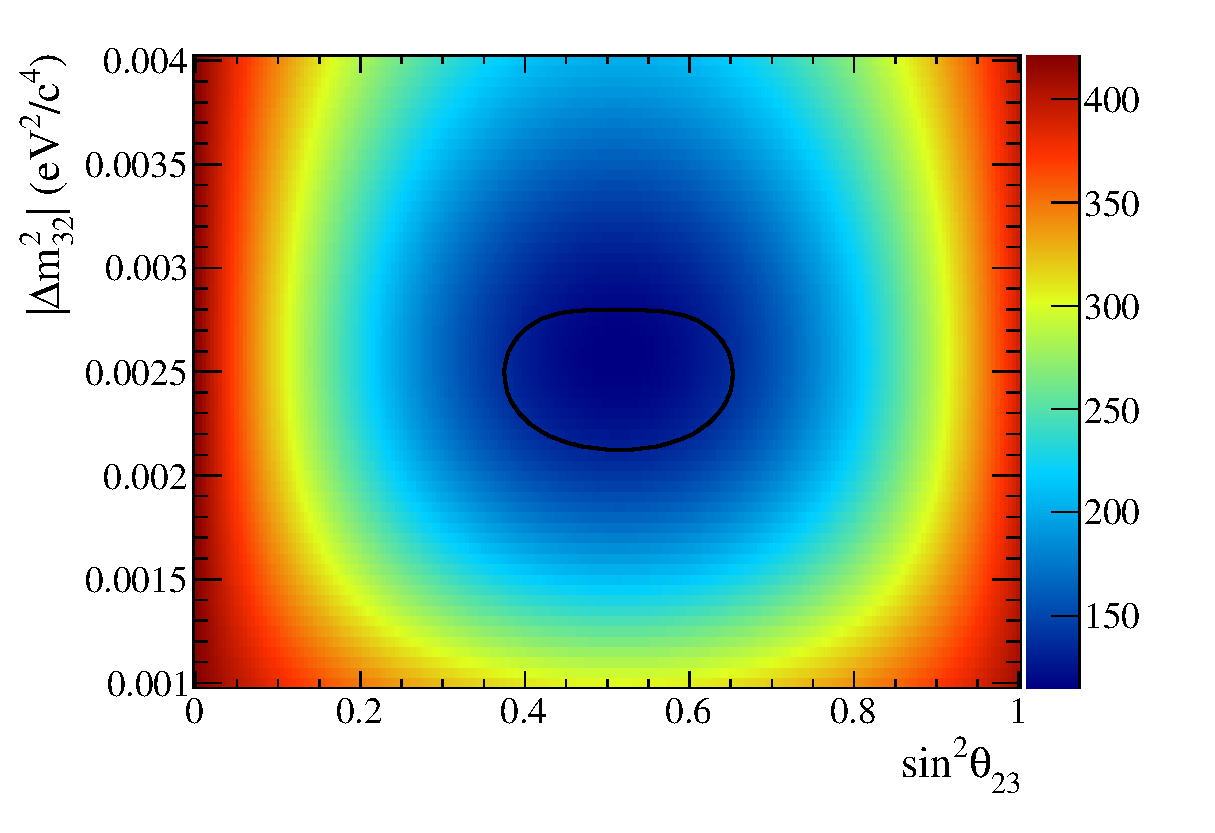
\includegraphics[width=32pc]{./images/spectrum_predictions/nsk_nominalbanff}
\caption {
  Predicted number of 1-ring $\mu$-like events,
  as a function of $\sin^{2}\theta_{23}$ and $|\Delta m^{2}_{32}|$,
  for an exposure of 6.3933$\times$10$^{20}$ POT.
  The number of events was calculated using the BANFF-tuned MC templates.
  Values shown in Tab. \ref{tab:pdg2012non23} are used for $\sin^{2}\theta_{13}$, $\sin^{2}\theta_{12}$ and $\Delta m^{2}_{21}$ and $\delta_{CP}$=0.
  The numbers shown were generated assuming the normal hierarchy.
  The T2K Run 1+2+3 90\% CL region is superimposed for reference.
}
\label{fig:nsk_vs_osc_params_tuned_mc}
\end{figure*}

%...........
%
% spectra, various osc scenarios
%
\begin{figure*}[htb]
\begin{minipage}[t]{0.48\linewidth}
\center
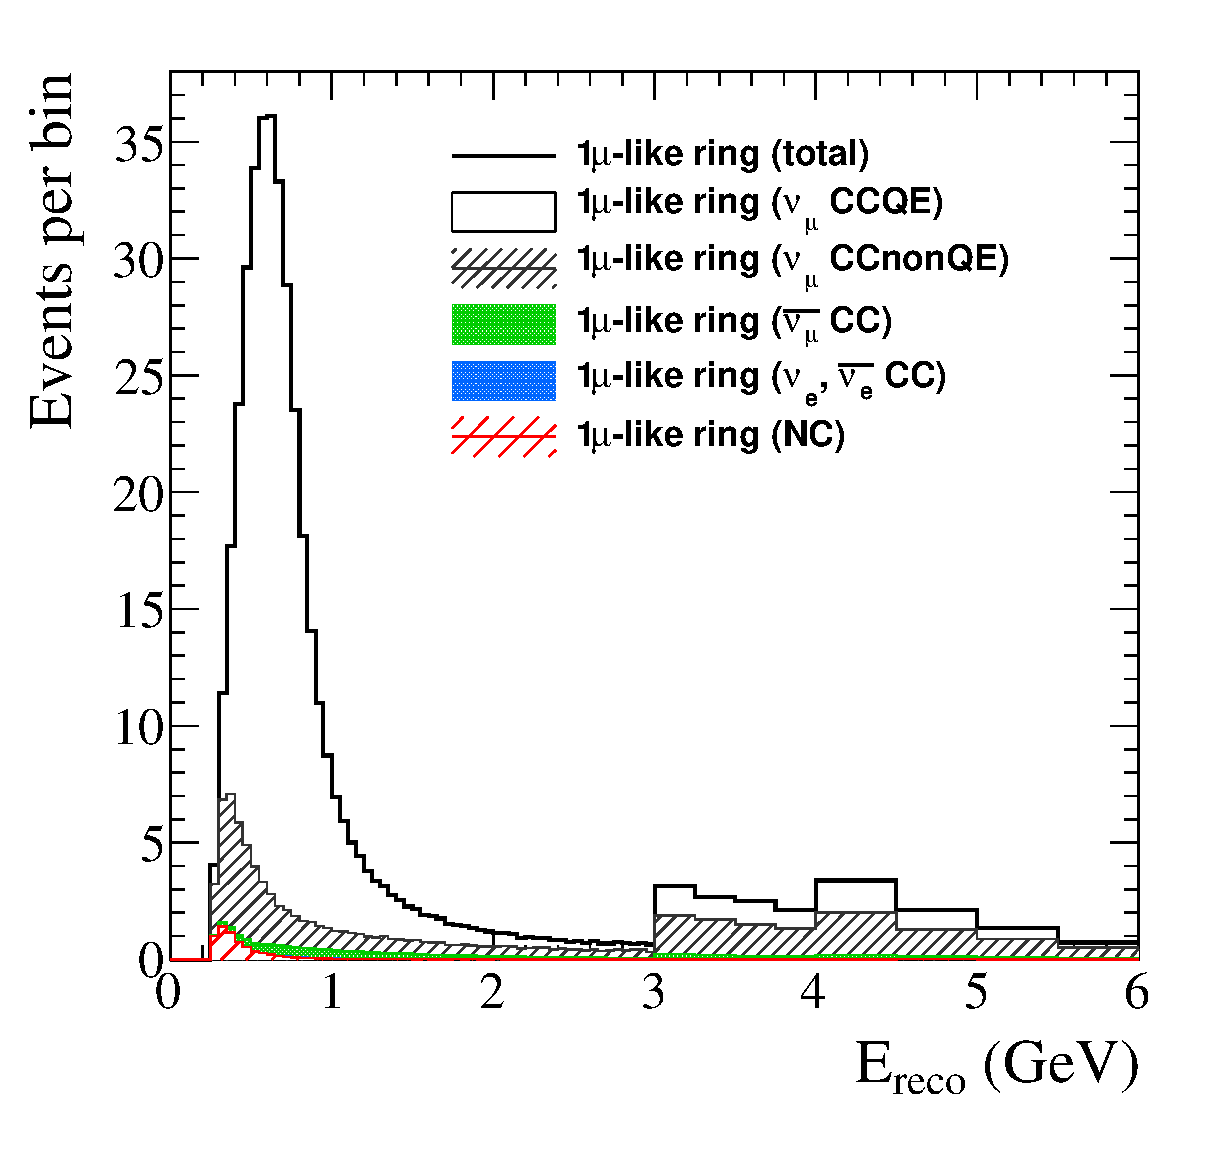
\includegraphics[width=20pc]{./images/spectrum_predictions/spectrum_breakdown_notoscillated_normal}
\caption {
Predicted reconstructed-energy spectrum of 1-ring $\mu$-like events,
and contributions from various true neutrino reaction modes,
for no oscillations and
for an exposure of 6.3933$\times$10$^{20}$ POT.
The 32 components of the spectrum are calculated separately in the actual analysis,
but, for this plot, are grouped into just 5 categories:
$\nu_{\mu}$ CCQE, $\nu_{\mu}$ CCnonQE, $\bar{\nu_{\mu}}$ CC, $\nu_{e}$/$\bar{\nu_{e}}$ CC and NC.
The spectrum was generated using the BANFF-tuned MC templates.
}
\label{fig:1Rmu_spectrum_and_components_no_osc}
\end{minipage}
\hspace{0.06\linewidth}
\begin{minipage}[t]{0.48\linewidth}
\center
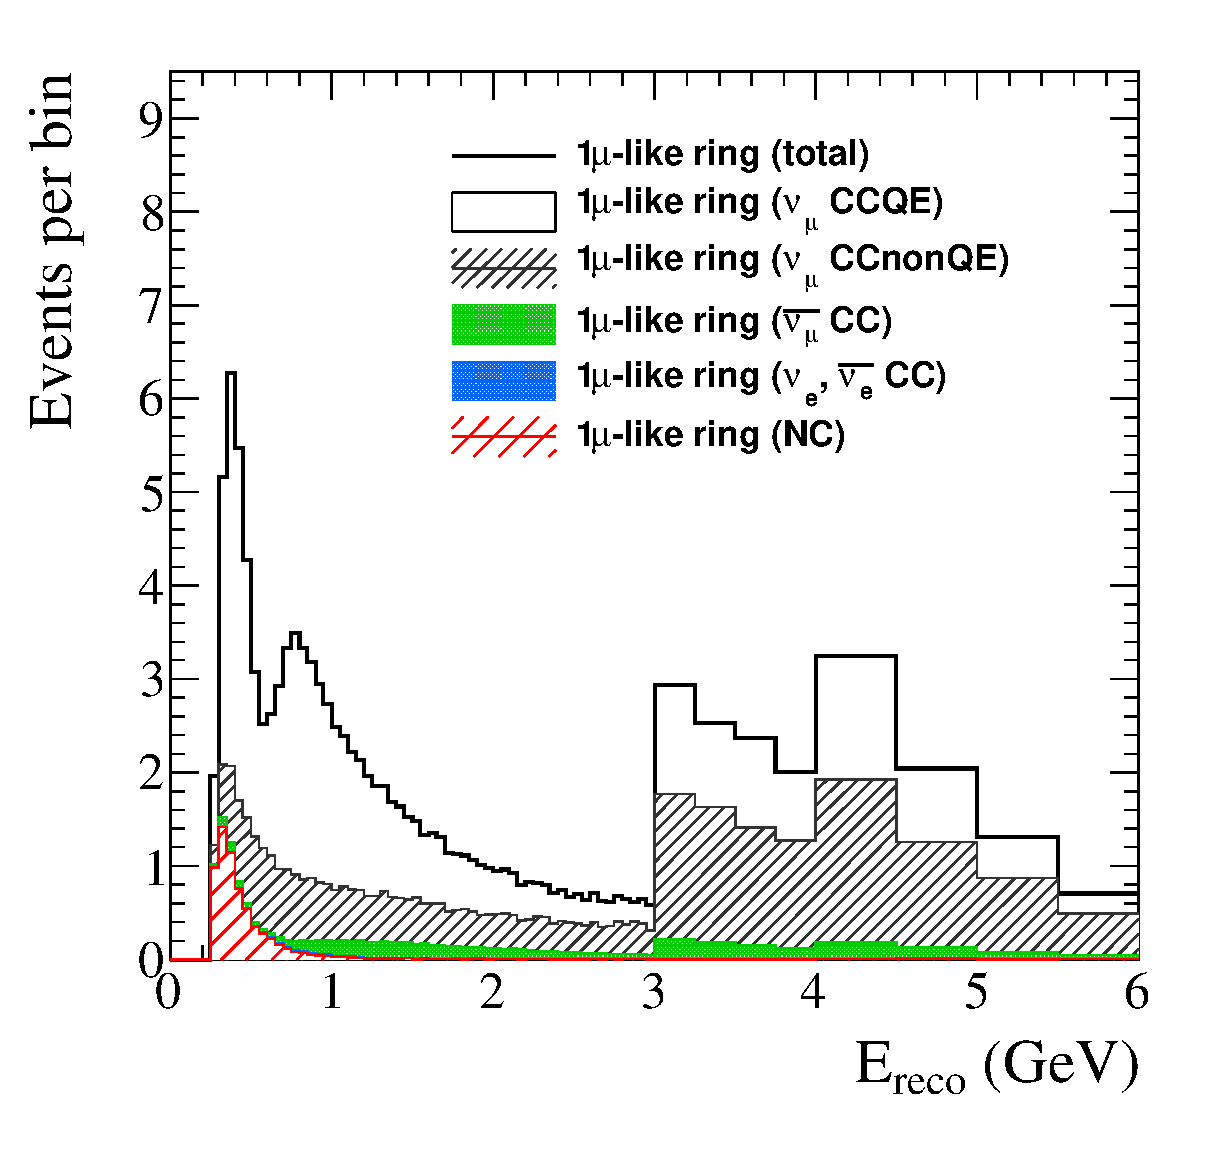
\includegraphics[width=20pc]{./images/spectrum_predictions/spectrum_breakdown_oscillated_normal}
\caption {
Predicted reconstructed-energy spectrum of 1-ring $\mu$-like events,
and contributions from various true neutrino reaction modes,
for oscillations with $\sin^{2}\theta_{23}$=0.5 and $|\Delta m^{2}_{32}|$=2.4$\times10^{-3}$ eV$^{2}$/c$^{4}$
and for an exposure of 6.3933$\times$10$^{20}$ POT.
The spectrum was generated using the BANFF-tuned MC templates.
Values shown in Tab. \ref{tab:pdg2012non23} are used for $\sin^{2}\theta_{13}$, $\sin^{2}\theta_{12}$ and $\Delta m^{2}_{21}$ and $\delta_{CP}$=0.
The spectrum shown was generated assuming the normal hierarchy.
Note that the vertical axis is zoomed in by a factor of 4 compared with Fig.\ \ref{fig:1Rmu_spectrum_and_components_no_osc}.
}
\label{fig:1Rmu_spectrum_and_components_default_osc}
\end{minipage}
\end{figure*}

%...........
%
% effect of tunes on nsk
%
\begin{figure*}[htb]
\begin{minipage}[t]{0.48\linewidth}
\center
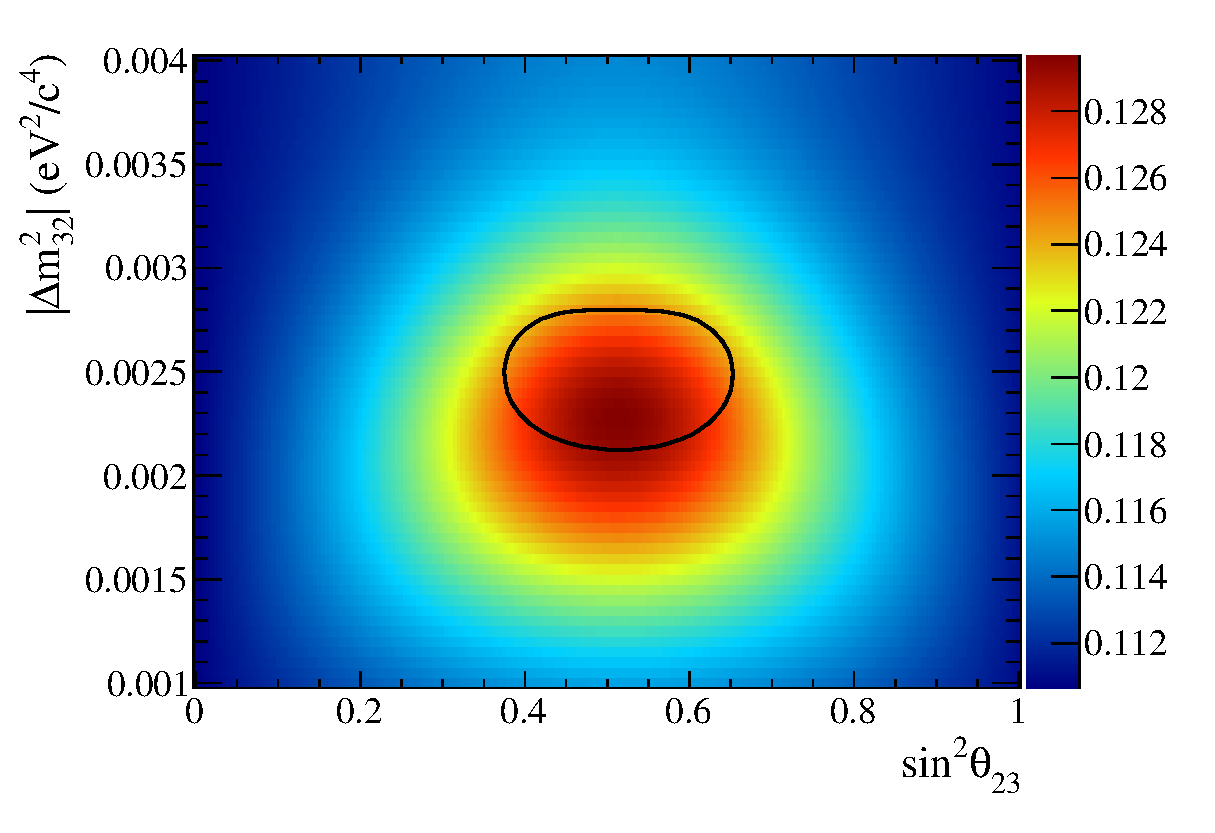
\includegraphics[width=18pc]{./images/spectrum_predictions/nsk_diff_nomflux}
\caption {
  Fractional difference in the predicted number of 1-ring $\mu$-like events
  as a result of applying the NA61 flux tuning to the nominal MC templates.
  This number is shown as a function of $\sin^{2}\theta_{23}$ and $|\Delta m^{2}_{32}|$
  for an exposure of 6.3933$\times$10$^{20}$ POT.
  Values shown in Tab. \ref{tab:pdg2012non23} are used for $\sin^{2}\theta_{13}$, $\sin^{2}\theta_{12}$ and $\Delta m^{2}_{21}$,and $\delta_{CP}$=0.
  The numbers shown were generated assuming the normal hierarchy.
  The T2K Run 1+2+3 90\% CL region is superimposed for reference.
}
\label{fig:nsk_vs_osc_params_effect_of_na61_tune}
\end{minipage}
\hspace{0.06\linewidth}
\begin{minipage}[t]{0.48\linewidth}
\center
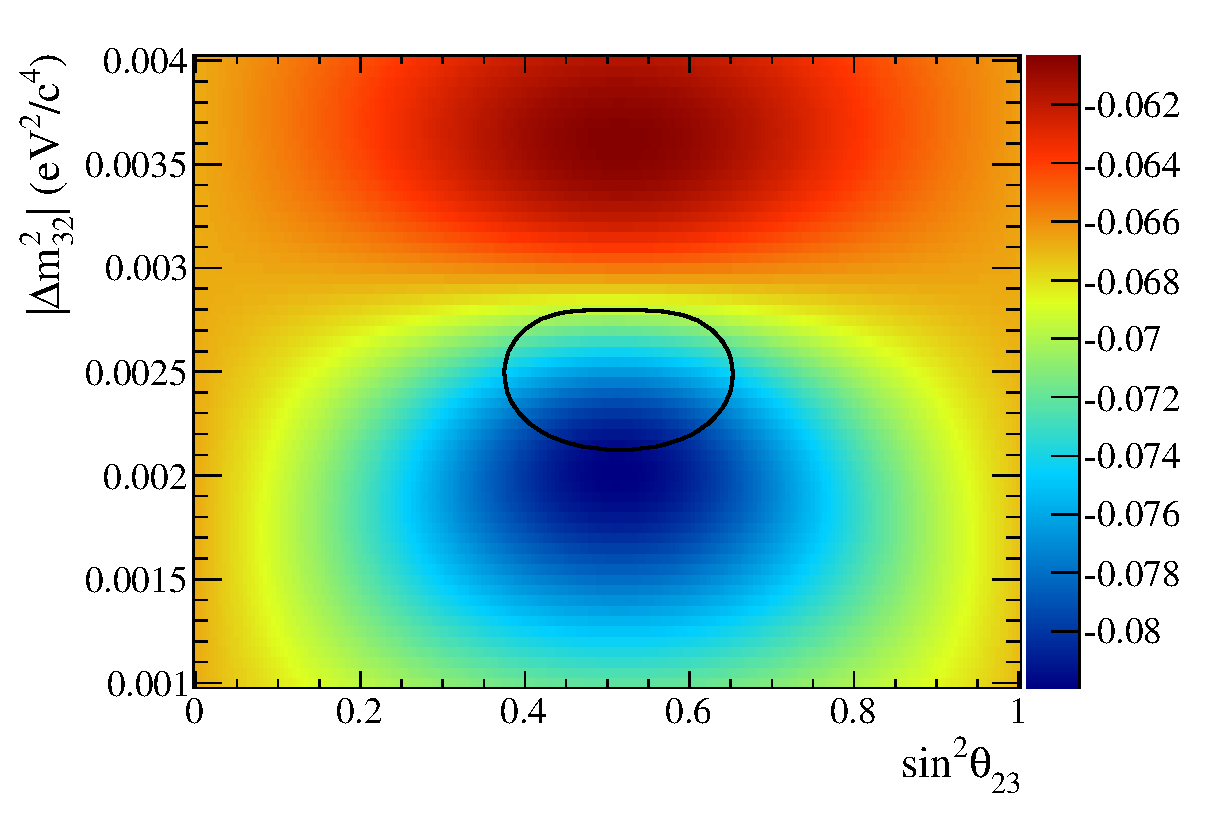
\includegraphics[width=18pc]{./images/spectrum_predictions/nsk_diff_tunflux}
\caption {
  Fractional difference in the predicted number of 1-ring $\mu$-like events
  as a result of applying the BANFF flux and cross-section tuning to the NA61 flux tuned MC templates.
  This number is shown as a function of $\sin^{2}\theta_{23}$ and $|\Delta m^{2}_{32}|$ and
  for an exposure of 6.3933$\times$10$^{20}$ POT.
  The values shown in Tab. \ref{tab:pdg2012non23} are used for $\sin^{2}\theta_{13}$, $\sin^{2}\theta_{12}$ and $\Delta m^{2}_{21}$, and $\delta_{CP}$=0.
  The numbers shown were generated assuming the normal hierarchy.
  The T2K Run 1+2+3 90\% CL region is superimposed for reference.
}
\label{fig:nsk_vs_osc_params_effect_of_banff_tune}
\end{minipage}
\end{figure*}

%...........
%
% tables showing the effect of tunes on nsk and nsk components
%
\begin{table}
\centering
\begin{tabular}{| c | c | c | c | }
\hline
                                                     & $N_{SK}$     & $N_{SK}$          & $N_{SK}$          \\
                                                     & (nominal MC) & (NA61-tuned MC)  & (BANFF-tuned MC)  \\
\hline
Total                                                  & 406.885590   & 451.896983  & 421.761456 \\
\hline
$\nu_\mu$ CCQE                                         & 323.303195   & 357.193543  & 333.937255 \\
$\nu_\mu$ CC 1$\pi$                                    &  54.678985   &  61.910123  &  57.152003 \\
$\nu_\mu$ CC coherent                                  &   1.845439   &   2.080564  &   2.040598 \\
$\nu_\mu$ CC other                                     &   7.748844   &   9.367262  &   9.303195 \\
$\nu_\mu$/$\nu_\tau$ NC 1$\pi^{+/-}$                   &   3.312363   &   3.790767  &   2.837281 \\
$\nu_\mu$/$\nu_\tau$ NC other                          &   2.833863   &   3.344421  &   3.123164 \\
Oscillated $\nu_\mu$ CCQE                              &   0.000000   &   0.000000  &   0.000000 \\
Oscillated $\nu_\mu$ CC 1$\pi$                         &   0.000000   &   0.000000  &   0.000000 \\
Oscillated $\nu_\mu$ CC coherent                       &   0.000000   &   0.000000  &   0.000000 \\
Oscillated $\nu_\mu$ CC other                          &   0.000000   &   0.000000  &   0.000000 \\
$\bar{\nu}_{\mu}$ CCQE                                 &   8.765816   &   9.448778  &   8.979168 \\
$\bar{\nu}_{\mu}$ CC 1$\pi$                            &   2.831107   &   3.055314  &   2.817605 \\
$\bar{\nu}_{\mu}$ CC coherent                          &   0.416568   &   0.449246  &   0.450921 \\
$\bar{\nu}_{\mu}$ CC other                             &   0.505131   &   0.543629  &   0.530826 \\
$\bar{\nu}_{\mu}$/$\bar{\nu}_{\tau}$ NC 1$\pi^{+/-}$   &   0.183251   &   0.199530  &   0.138736 \\
$\bar{\nu}_{\mu}$/$\bar{\nu}_{\tau}$ NC other          &   0.171682   &   0.185494  &   0.169629 \\
$\nu_e$ CCQE                                           &   0.034418   &   0.037030  &   0.035433 \\
$\nu_e$ CC 1$\pi$                                      &   0.020994   &   0.023160  &   0.022092 \\
$\nu_e$ CC coherent                                    &   0.001028   &   0.001123  &   0.001123 \\
$\nu_e$ CC other                                       &   0.005655   &   0.006715  &   0.006598 \\
$\nu_e$ NC 1$\pi^{+/-}$                                &   0.088973   &   0.102385  &   0.073063 \\
$\nu_e$ NC other                                       &   0.109167   &   0.128465  &   0.118603 \\
$\bar{\nu}_{e}$ CCQE                                   &   0.002116   &   0.002127  &   0.001992 \\
$\bar{\nu}_{e}$ CC 1$\pi$                              &   0.001339   &   0.001346  &   0.001242 \\
$\bar{\nu}_{e}$ CC coherent                            &   0.000131   &   0.000134  &   0.000134 \\
$\bar{\nu}_{e}$ CC other                               &   0.000430   &   0.000434  &   0.000420 \\
$\bar{\nu}_{e}$ NC 1$\pi^{+/-}$                        &   0.011925   &   0.012072  &   0.008187 \\
$\bar{\nu}_{e}$ NC other                               &   0.013168   &   0.013319  &   0.012187 \\
Oscillated $\nu_e$ CCQE                                &   0.000000   &   0.000000  &   0.000000 \\
Oscillated $\nu_e$ CC 1$\pi$                           &   0.000000   &   0.000000  &   0.000000 \\
Oscillated $\nu_e$ CC coherent                         &   0.000000   &   0.000000  &   0.000000 \\
Oscillated $\nu_e$ CC other                            &   0.000000   &   0.000000  &   0.000000 \\
\hline
\end{tabular}
\caption{
  Calculated numbers of 1-ring $\mu$-like events without oscillations using the nominal MC templates, the
  NA61-tuned MC templates and the BANFF-tuned MC templates.
  The total numbers of events and the numbers of events from each mode considered in this analysis are shown.
  These numbers were calculated for an exposure of 6.3933$\times$10$^{20}$ POT.
}
\label{tab:nsk_nominal_x3_no_osc}
\end{table}


\begin{table}
\centering
\begin{tabular}{| c | c | c | c | }
\hline
                                                     & $N_{SK}$     & $N_{SK}$         & $N_{SK}$          \\
                                                     & (nominal MC) & (NA61-tuned MC)  & (BANFF-tuned MC)  \\
\hline
Total                                                & 113.170201   & 127.802057       & 117.776282 \\
\hline
$\nu_\mu$ CCQE                                       &  64.362490   &  71.563162       &  67.144118 \\
$\nu_\mu$ CC 1$\pi$                                  &  26.993670   &  31.161684       &  27.453878 \\
$\nu_\mu$ CC coherent                                &   0.756691   &   0.874092       &   0.879517 \\
$\nu_\mu$ CC other                                   &   6.882348   &   8.377876       &   8.317477 \\
$\nu_\mu$/$\nu_\tau$ NC 1$\pi^{+/-}$                 &   3.312363   &   3.790767       &   2.837281 \\
$\nu_\mu$/$\nu_\tau$ NC other                        &   2.833863   &   3.344421       &   3.123164 \\
Oscillated $\nu_\mu$ CCQE                            &   0.114233   &   0.126452       &   0.121548 \\
Oscillated $\nu_\mu$ CC 1$\pi$                       &   0.026640   &   0.029728       &   0.028577 \\
Oscillated $\nu_\mu$ CC coherent                     &   0.000799   &   0.000890       &   0.000890 \\
Oscillated $\nu_\mu$ CC other                        &   0.002280   &   0.002583       &   0.002545 \\
$\bar{\nu}_{\mu}$ CCQE                               &   4.310464   &   4.655209       &   4.351636 \\
$\bar{\nu}_{\mu}$ CC 1$\pi$                          &   2.024431   &   2.180599       &   1.967334 \\
$\bar{\nu}_{\mu}$ CC coherent                        &   0.222639   &   0.240227       &   0.240845 \\
$\bar{\nu}_{\mu}$ CC other                           &   0.448188   &   0.481943       &   0.470039 \\
$\bar{\nu}_{\mu}$/$\bar{\nu}_{\tau}$ NC 1$\pi^{+/-}$ &   0.183251   &   0.199530       &   0.138736 \\
$\bar{\nu}_{\mu}$/$\bar{\nu}_{\tau}$ NC other        &   0.171682   &   0.185494       &   0.169629 \\
$\nu_e$ CCQE                                         &   0.031971   &   0.034415       &   0.032912 \\
$\nu_e$ CC 1$\pi$                                    &   0.019924   &   0.022017       &   0.020920 \\
$\nu_e$ CC coherent                                  &   0.000961   &   0.001050       &   0.001050 \\
$\nu_e$ CC other                                     &   0.005562   &   0.006611       &   0.006496 \\
$\nu_e$ NC 1$\pi^{+/-}$                              &   0.088973   &   0.102385       &   0.073063 \\
$\nu_e$ NC other                                     &   0.109167   &   0.128465       &   0.118603 \\
$\bar{\nu}_{e}$ CCQE                                 &   0.002029   &   0.002039       &   0.001908 \\
$\bar{\nu}_{e}$ CC 1$\pi$                            &   0.001301   &   0.001308       &   0.001204 \\
$\bar{\nu}_{e}$ CC coherent                          &   0.000127   &   0.000130       &   0.000130 \\
$\bar{\nu}_{e}$ CC other                             &   0.000426   &   0.000431       &   0.000417 \\
$\bar{\nu}_{e}$ NC 1$\pi^{+/-}$                      &   0.011925   &   0.012072       &   0.008187 \\
$\bar{\nu}_{e}$ NC other                             &   0.013168   &   0.013319       &   0.012187 \\
Oscillated $\nu_e$ CCQE                              &   0.174872   &   0.192606       &   0.180557 \\
Oscillated $\nu_e$ CC 1$\pi$                         &   0.057775   &   0.063921       &   0.064998 \\
Oscillated $\nu_e$ CC coherent                       &   0.004620   &   0.005090       &   0.004929 \\
Oscillated $\nu_e$ CC other                          &   0.001368   &   0.001539       &   0.001508 \\
\hline
\end{tabular}
\caption{
  Calculated numbers of 1-ring $\mu$-like events using the nominal MC templates, the NA61-tuned MC templates
  and the BANFF-tuned MC templates.
  The total numbers of events and the numbers of events from each mode considered in this analysis are shown.
  These numbers were calculated for an exposure of 6.3933$\times$10$^{20}$ POT 
  and oscillations with $\sin^{2}\theta_{23}$=0.5 and $|\Delta m^{2}_{32}|$=2.4$\times$10$^{-3}$ eV$^{2}$/c$^{4}$.
  Values shown in Tab. \ref{tab:pdg2012non23} are used for $\sin^{2}\theta_{13}$, $\sin^{2}\theta_{12}$ and $\Delta m^{2}_{21}$ and $\delta_{CP}$=0.
  The normal hierarchy is assumed.
}
\label{tab:nsk_nominal_x3_default_osc}
\end{table}


%...........
%
% Plots showing the effect of tunes on Ereco spectra
%
\begin{figure*}[htb]
\center
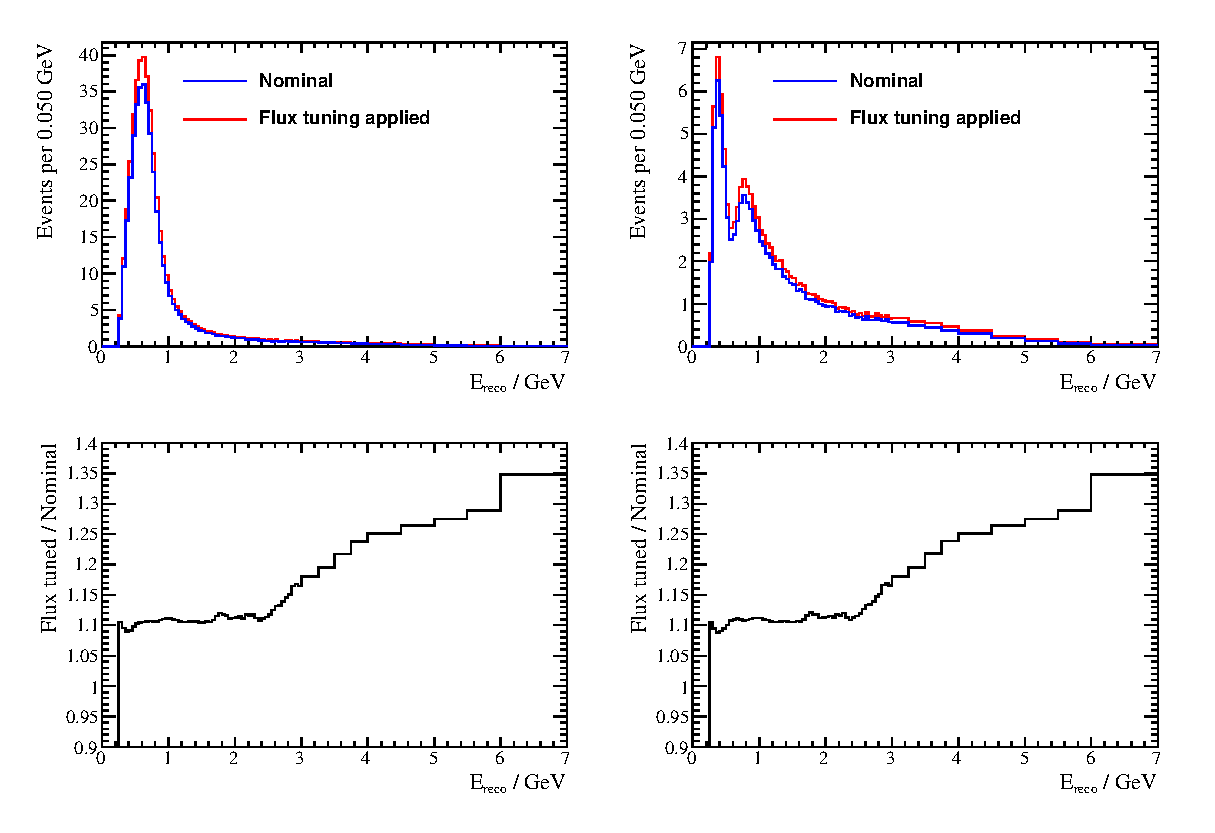
\includegraphics[width=30pc]{./images/spectrum_predictions/spectra_nom_fluxtuned}
\caption {
Reconstructed-energy spectrum of 1-ring $\mu$-like events,
for an exposure of 6.3933$\times$10$^{20}$ POT,
both with and without the effect of the NA61 flux tuning of the nominal MC templates.
The spectra are shown both for no oscillations (left)
and for oscillations with $\sin^{2}\theta_{23}$=0.5, $|\Delta m^{2}_{32}|$=2.4$\times$10$^{-3}$ eV$^{2}$/c$^{4}$,
the 2012 PDG values for $\sin^{2}\theta_{13}$, $\sin^{2}\theta_{12}$ and $\Delta m^{2}_{21}$, and
$\delta_{CP}$=0 (right). Results shown for the normal hierarchy.
}
\label{fig:1Rmu_spectrum_w_and_wo_na61_weights}
\end{figure*}

\begin{figure*}[htb]
\center
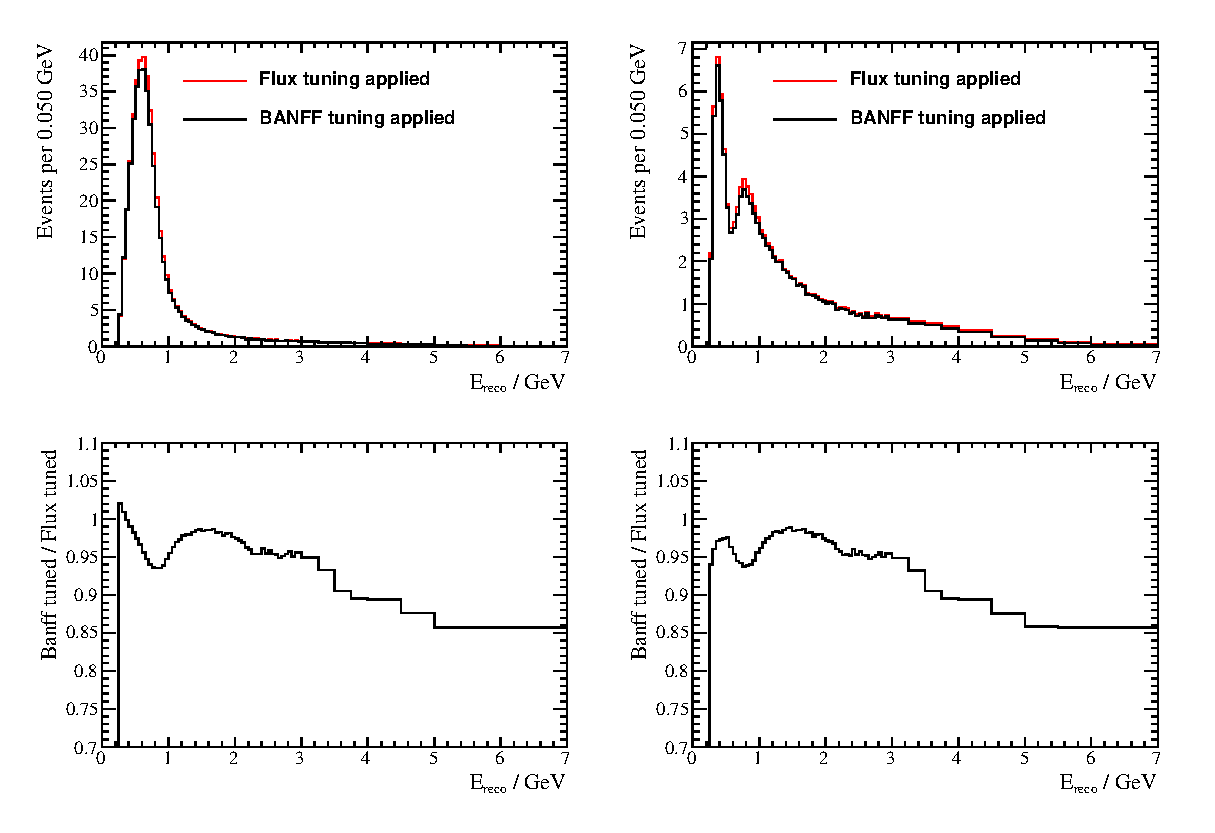
\includegraphics[width=30pc]{./images/spectrum_predictions/spectra_tun_banfftuned}
\caption {
Reconstructed-energy spectrum of 1-ring $\mu$-like events,
for an exposure of 6.3933$\times$10$^{20}$ POT,
both with and without the effect of BANFF flux and cross-section tuning on the NA61-tuned flux MC templates.
The spectra are shown both for no 23-sector oscillations (left)
and for oscillations with $\sin^{2}\theta_{23}$=0.5 and $|\Delta m^{2}_{32}|$=2.4$\times$10$^{-3}$ eV$^{2}$/c$^{4}$ (right).
In all spectra, the 2012 PDG parameters are used for $\sin^{2}\theta_{13}$, $\sin^{2}\theta_{12}$ and $\Delta m^{2}_{21}$
and $\delta_{CP}$=0. Results shown for the normal hierarchy.
}
\label{fig:1Rmu_spectrum_w_and_wo_banff_weights}
\end{figure*}

%...........
%
% Effect of \emph{non-23-sector} params
% Effect of mass hierarchy
%
\begin{figure*}[htb]
\begin{minipage}[t]{0.48\linewidth}
\center
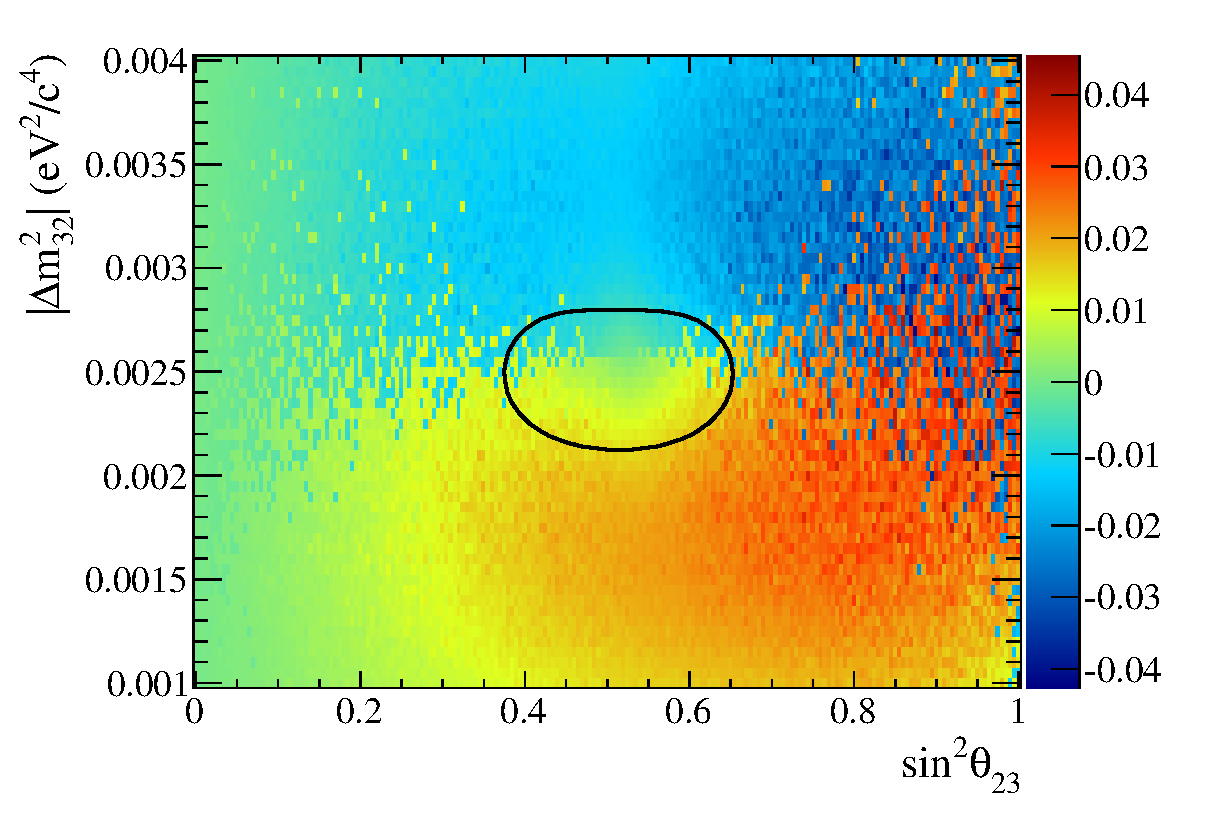
\includegraphics[width=18pc]{./images/spectrum_predictions/nsk_diff_non23throw}
\caption {
  Maximum value of the fractional difference in the predicted number of 1-ring $\mu$-like events
  between varying each of $\sin^{2}\theta_{13}$, $\sin^{2}\theta_{12}$, $\Delta m^{2}_{21}$ and $\delta_{CP}$
  within their allowed ranges and their nominal values (these are the values shown in Tab. \ref{tab:pdg2012non23} for $\sin^{2}\theta_{13}$,
  $\sin^{2}\theta_{12}$ and $\Delta m^{2}_{21}$, and $\delta_{CP}$=0).
  The fractional difference is shown as function of $\sin^{2}\theta_{23}$ and $|\Delta m^{2}_{32}|$,
  for an exposure of 6.3933$\times$10$^{20}$ POT.
  The number of events was calculated using the BANFF-tuned MC templates.
  The normal hierarchy was assumed.
  The T2K Run 1+2+3 90\% CL region is superimposed for reference.
}
\label{fig:nsk_vs_osc_params_tuned_mc_effect_of_non23}
\end{minipage}
\hspace{0.06\linewidth}
\begin{minipage}[t]{0.48\linewidth}
\center
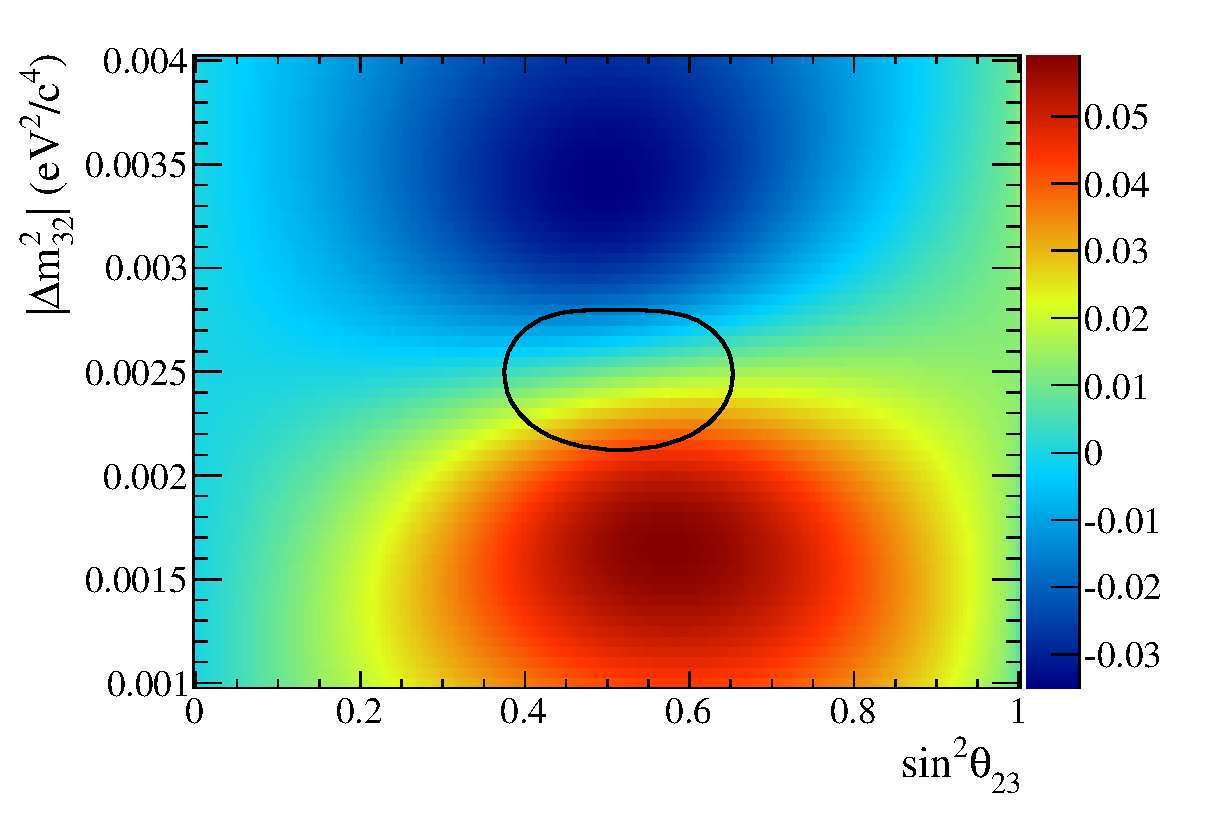
\includegraphics[width=18pc]{./images/spectrum_predictions/nsk_diff_inv}
\caption {
  Fractional difference in the predicted number of 1-ring $\mu$-like events between assuming the normal hierarchy
  and assuming the inverted hierarchy.
  The fractional difference is shown as function of $\sin^{2}\theta_{23}$ and $|\Delta m^{2}_{32}|$,
  for an exposure of 6.3933$\times$10$^{20}$ POT.
  The number of events was calculated using the BANFF-tuned MC templates.
  The values shown in Tab. \ref{tab:pdg2012non23} are used for $\sin^{2}\theta_{13}$, $\sin^{2}\theta_{12}$ and $\Delta m^{2}_{21}$, and $\delta_{CP}$=0.
  The T2K Run 1+2+3 90\% CL region is superimposed for reference.
}
\label{fig:nsk_vs_osc_params_tuned_mc_effect_of_hierarchy}
\end{minipage}
\end{figure*}

